\documentclass[tikz,border=2pt]{standalone}
\usepackage{amsmath,amssymb}
\usepackage{tikz}
\usetikzlibrary{arrows.meta}

\begin{document}
% Augmented form: every <= constraint becomes an equation by adding a nonnegative slack
% variable that measures the unused capacity.
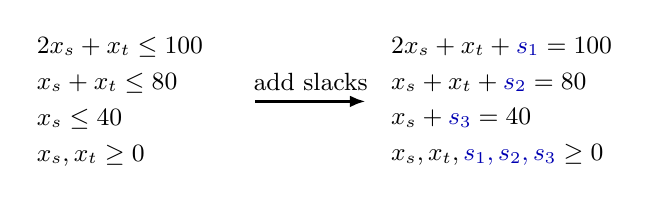
\begin{tikzpicture}[every node/.style={font=\small}, >={Latex[length=2mm]}]
	\node[anchor=west, align=left] at (0,0) {$2x_s+x_t\le100$\\[2pt] $x_s+x_t\le80$\\[2pt] $x_s\le40$\\[2pt] $x_s,x_t\ge0$};
	\draw[->, very thick] (2.9,0) -- (4.3,0) node[midway, above] {add slacks};
	\node[anchor=west, align=left] at (4.5,0) {$2x_s+x_t+\textcolor{blue!70!black}{s_1}=100$\\[2pt] $x_s+x_t+\textcolor{blue!70!black}{s_2}=80$\\[2pt] $x_s+\textcolor{blue!70!black}{s_3}=40$\\[2pt] $x_s,x_t,\textcolor{blue!70!black}{s_1,s_2,s_3}\ge0$};
	\end{tikzpicture}
\end{document}
